\section{Transformation to Dual}
\label{sect:implementation-transformation}

Thomassen \cite{thomassen1992plane} provides a strong theoretical result: place cubic graphs are area-universal, \ie{} they can be drawn with equivalent combinatorial embeddings and straight-line edges with arbitrary given face areas. Considering forming the boundary graph first adds a helper vertex in the outer face, turning the filtered graph in a fully triangulated graph, its dual is then a graph in which all vertices have degree 3. Therefore, according to Thomassen, we can form a contact representation with perfect statistical accuracy. The construction of such a contact representation is fairly complicated through and leaves us with very few \emdash{} in fact, the minimum possible number of \emdash{} vertices in the boundary graph. With so little vertices and thus little degrees of freedoms, it is close to impossible to create regions that fit our aesthetic criteria.
% Kleist will only appear in Future Work when relaxing requirements.

We therefore propose a simple algorithm that is trivial to implement and leaves us with twice the number of degrees of freedom as shown. However, it can easily be adapted to created as many degrees of freedom as required.

The underlying idea is as follows: We place vertices on edges of the outer face (those edges form new triangular faces after adding the helper vertex from \cref{sect:transformation-to-dual}) and inside the internal faces. We then connect these vertices if their corresponding faces are incident. Connecting two vertices may require additional subdivision vertices in order not to introduce edge crossings \emdash{} we use a single subdivision vertex per edge.

In a preliminary step, we tweak the embedding of the filtered graph to use straight-line edges. Such an embedding exists for every plane graph according to Fáry's theorem \cite{fary1948straight} and was independently proved by Wagner \cite{wagner1936bemerkungen} and Stein \cite{stein1951convex}. There exist numerous algorithms to construct such an embedding \cite{vismara} such as the shift method \cite{fraysseix1990draw} or the Schnyder realizer method \cite{schnyder1990embedding} \todo{Tamara mentioned a very simple algorithm with exponential area?}.

\clearpage
\begin{algorithm}[H]
  \caption{Transformation to Dual}
  \label{algo:transformation-to-dual}
  \SetKwData{Endpoints}{endpoints}
  \SetKwFunction{Appending}{appending}
  \SetArgSty{textrm}
  \vspace{5pt}
  \KwData{$G_\text{in}$: planar straight-line embedding of 2-connected, internally triangulated graph}
  \KwResult{$G_\text{out}$: planar straight-line embedding of 1-subdivision of augmented dual of $G_\text{in}$}
  \vspace{10pt}
  create empty output graph $G_\text{out}$\;
  \ForEach{inner face $f$ in $G_\text{in}$}{
    \label{line:transformation-loop1-start}
    add \quoted{inner face vertex} $v_f$ to $G_\text{out}$\;
    position $v_f$ at barycenter of $f$ in $G_\text{in}$ \label{line:transformation-barycenter1}\;
    \label{line:transformation-loop1-end}
  }
  \ForEach{edge $\{u,v\}$ in $G_\text{in}$}{
    \label{line:transformation-loop2-start}
  	\If{$\{u,v\}$ is incident to two different faces $f, g$ in $G_\text{in}$ \label{line:transformation-incidentfacelookup1}}{
  	  add \quoted{subdivision vertex} $v_\text{sub}$ to $G_\text{out}$\;
  	  position $v_\text{sub}$ at midpoint of ${\{u,v\}}$ in $G_\text{in}$\;
  	  add edge between $v_f$ and $v_\text{sub}$ to $G_\text{out}$\;
  	  add edge between $v_\text{sub}$ and $v_g$ to $G_\text{out}$\;
  	}
  	\ElseIf{$\{u,v\}$ is incident to a single face $f$ in $G_\text{in}$ \label{line:transformation-incidentfacelookup2}}{
  	  add \quoted{outer edge vertex} $v_{\{u,v\}}$ to $G_\text{out}$\;
  	  position $v_{\{u,v\}}$ at midpoint of ${\{u,v\}}$ in $G_\text{in}$\;
  	  add \quoted{subdivision vertex} $v_\text{sub}$ to $G_\text{out}$\;
  	  position $v_\text{sub}$ at midpoint of barycenter of $f$ and midpoint of ${\{u,v\}}$ in $G_\text{in}$ \label{line:transformation-barycenter2}\;
  	  add edge between $v_{\{u,v\}}$ and $v_\text{sub}$ to $G_\text{out}$\;
  	  add edge between $v_\text{sub}$ and $v_f$ to $G_\text{out}$\;
  	}
  	\label{line:transformation-loop2-end}
  }
  \ForEach{incident edges $\{\{u,v\},\{v,w\}\}$ on outer face of $G_\text{in}$}{
    \label{line:transformation-loop3-start}
    add \quoted{subdivision vertex} $v_\text{sub}$ to $G_\text{out}$\;
    position $v_\text{sub}$ at position of $v$ in $G_\text{in}$\;
    add edge between $v_{\{u,v\}}$ and $v_\text{sub}$ to $G_\text{out}$\;
    add edge between $v_\text{sub}$ and $v_{\{v,w\}}$ to $G_\text{out}$\;
    \label{line:transformation-loop3-end}
  }
  \ForEach{vertex $u$ in $G_\text{in}$ \label{line:transformation-enumeratevertices}}{
    \label{line:transformation-loop4-start}
    $\Endpoints \gets ()$\;
    \ForEach{adjacent pair $(v,w)$ of neighbors of $u$ (according to embedding) \label{line:transformation-enumerateedges}}{
      \If{$u,v,w$ is a triangular face $f$ with positive area in $G_\text{in}$ \label{line:transformation-checktriangle}}{
        append $v_f$ to \Endpoints\;
      }
      \Else{
        append $v_{\{u,v\}}$ to \Endpoints\;
        append $v_{\{u,w\}}$ to \Endpoints\;
      }
    }
    \ForEach{adjacent pair $(v,w)$ in \Endpoints}{
      insert subdivision vertex connecting $v$ to $w$ between $v$ and $w$ in \Endpoints\;
    }
    define $f_u$ as face on \Endpoints\;
    set weight of $f_u$ to weight of $u$ in $G_\text{in}$\;
    \label{line:transformation-loop4-end}
  }
  \ForEach{edge $\{u,v\}$ in $G_\text{in}$}{
    \label{line:transformation-loop5-start}
    set weight of adjacency between $f_u$ and $f_v$ to weight of $\{u,v\}$ in $G_\text{in}$\;
    \label{line:transformation-loop5-end}
  }
  \Return $G_\text{out}$
\end{algorithm}

\paragraph{Correctness}
\lipsum

\begin{figure}[H]
	\centering
	\subfigure[$G_\text{in}$]{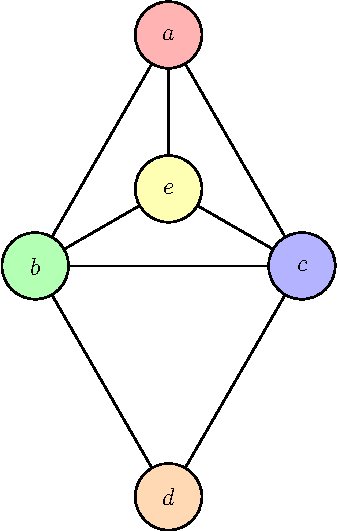
\includegraphics[height=70mm]{Resources/Implementation-Transformation-Primal.pdf}}
	\quad
	\subfigure[$G_\text{out}$]{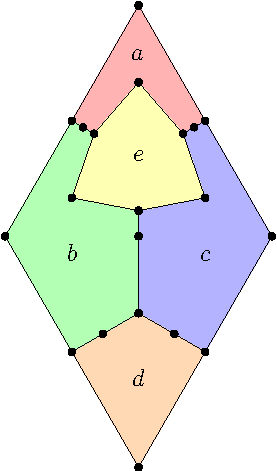
\includegraphics[height=70mm]{Resources/Implementation-Transformation-Dual.pdf}}
	\caption{An embedded filtered graph (a) and its dual as produced by \cref{algo:transformation-to-dual} (b).}
	\label{fig:implementation-transformation}
\end{figure}

\paragraph{Runtime}

To compute the input graph's faces, we replace every edge with two inversely oriented, directed edges. We then repeatedly pick any unmarked edge and form a directed cycle by following the next outgoing edge according to the embedding, marking the edges as we go. Once all edges have been marked, we have found all faces. The outer face is the only face with negative area. This can be implemented in $\bigTheta{\abs{V_\text{in}} + \abs{E_\text{in}}}$.

The input graph has $\bigTheta{\abs{V_\text{in}}}$ internal faces and they are all triangles, therefore we can compute their barycenter in $\bigTheta{1}$ each (\cref{line:transformation-barycenter1}, \cref{line:transformation-barycenter2}). By keeping track of of which faces an edge of the input graph is incident to while computing the faces as outlined above, we allow for $\bigTheta{1}$ lookups in \cref{line:transformation-incidentfacelookup1} and \cref{line:transformation-incidentfacelookup2}. The loop in \crefrange{line:transformation-loop1-start}{line:transformation-loop1-end} therefore runs in $\bigTheta{\abs{V_\text{in}}}$, the loop in \crefrange{line:transformation-loop2-start}{line:transformation-loop2-end} in $\bigTheta{\abs{E_\text{in}}}$, and the loop in \crefrange{line:transformation-loop3-start}{line:transformation-loop3-end} in $\bigTheta{\abs{E_\text{in}}}$.

The loop in \crefrange{line:transformation-loop4-start}{line:transformation-loop4-end} processes every vertex once in \cref{line:transformation-enumeratevertices} and and every edge twice \cref{line:transformation-enumerateedges}. We can check if the vertices $u,v,w$ form a triangle in constant time (\cref{line:transformation-checktriangle}) by checking if there's an edge between $v$ and $w$. Considering each of the $\bigTheta{\abs{V_\text{in}} + \abs{E_\text{in}}}$ vertices of the generated graph appears in \code{endpoints} in no more than two iterations of the loop in \crefrange{line:transformation-loop4-start}{line:transformation-loop4-end} and all those vertices have degree 3, we can find their shared neighbor in constant time and implement the entire loop to run in $\bigTheta{\abs{V_\text{in}} + \abs{E_\text{in}}}$.

By keeping track of which faces in the generated graph correspond to which vertices in the source graph in \crefrange{line:transformation-loop4-start}{line:transformation-loop4-end}, the loop in \crefrange{line:transformation-loop5-start}{line:transformation-loop5-end} runs in $\bigTheta{\abs{V_\text{in}} + \abs{E_\text{in}}}$.

The entire algorithm can therefore be implemented to run in $\bigTheta{\abs{V_\text{in}} + \abs{E_\text{in}}}$.
